%%%%%%%%%%%%%%%%%%%%%%%%%%%%%%%%%%%%%%%%%%%%%%%%%%%%%%%%%%%%%%%%%%%%%%%%%%%%%%%%
%2345678901234567890123456789012345678901234567890123456789012345678901234567890
%        1         2         3         4         5         6         7         8

\documentclass[letterpaper, 10 pt, conference]{ieeeconf}  % Comment this line out if you need a4paper

%\documentclass[a4paper, 10pt, conference]{ieeeconf}      % Use this line for a4 paper

\IEEEoverridecommandlockouts                              % This command is only needed if you want to use the \thanks command

\overrideIEEEmargins                                      % Needed to meet printer requirements.

% See the \addtolength command later in the file to balance the column lengths
% on the last page of the document

% The following packages can be found on http:\\www.ctan.org
\usepackage{graphicx} % for pdf, bitmapped graphics files
%\usepackage{epsfig} % for postscript graphics files
%\usepackage{mathptmx} % assumes new font selection scheme installed
%\usepackage{times} % assumes new font selection scheme installed
%\usepackage{amsmath} % assumes amsmath package installed
%\usepackage{amssymb}  % assumes amsmath package installed

\title{\LARGE \bf
% Preparation of Papers for IEEE Sponsored Conferences \& Symposia*
Movie Rating Predictor Using Nonnegative Matrix Factorization on Tag Data
}


\author{Claire Chang, Thaxter Shaw, and TJ Tsai$^{1}$% <-this % stops a space
\thanks{$^{1}$T. Tsai is with the Department of Engineering at Harvey Mudd College,
301 Platt Blvd., Claremont, CA 91711. E-mail: {\tt\small ttsai@hmc.edu}}%
}



\begin{document}



\maketitle
\thispagestyle{empty}
\pagestyle{empty}


%%%%%%%%%%%%%%%%%%%%%%%%%%%%%%%%%%%%%%%%%%%%%%%%%%%%%%%%%%%%%%%%%%%%%%%%%%%%%%%%
\begin{abstract}

The goal of recommendation systems is to suggest suitable content such as movies, groceries, and more. This article aims to predict what someone will rate a movie, which could in turn be applied to a movie recommendation system. We propose a method of addressing this problem 

\end{abstract}


%%%%%%%%%%%%%%%%%%%%%%%%%%%%%%%%%%%%%%%%%%%%%%%%%%%%%%%%%%%%%%%%%%%%%%%%%%%%%%%%
\section{INTRODUCTION}

The goal of this paper is to predict what someone will rate a movie on a five-star scale.
This prediction can be used in recommendation systems (citation?) for not only movies, but also grocery shopping, music, and more.

There are several obstacles that make this problem challenging. 
One issue, as investigated in [citation Netflix Bellsmth] is the effect of time. Over time, users may change their baseline rating (for example, have higher expectations of graphics) and begin to prefer different genres and actors.
Movies themselves also become more or less popular over time.

One approach that has been taken is to use a "neighborhood approach" that compares different movies, and recommends a highly rated movie that is similar to other movies a user has liked [citation]. 
Another approach is to use collaborative filtering (CF) methods (citation) such as nonnegative matrix factorization (NMF) and singular value decomposition (SVD). 
We could also use a hybrid approach of the neighborhood and CF approahces [citation Koren 2008].

In this paper, we use data from MovieLens [citation]. The dataset we use contains ratings of over 1000 movies made by various users, filtered such that each user has rated at least 20 movies.
The dataset also relates each movie to a series of short tags, such as "sci-fi," "cliché," or "overrated." This data was collected through users applying labels to movies, and machine learning [citation Tag Genome].

Our system uses NMF on this tag data to create clusters of tags, which we will equate to "genres". We then use these genres predict ratings. Finally, we use mean movie ratings to adjust this predicted rating.


\section{SYSTEM DESCRIPTION}

\begin{figure}[h]
   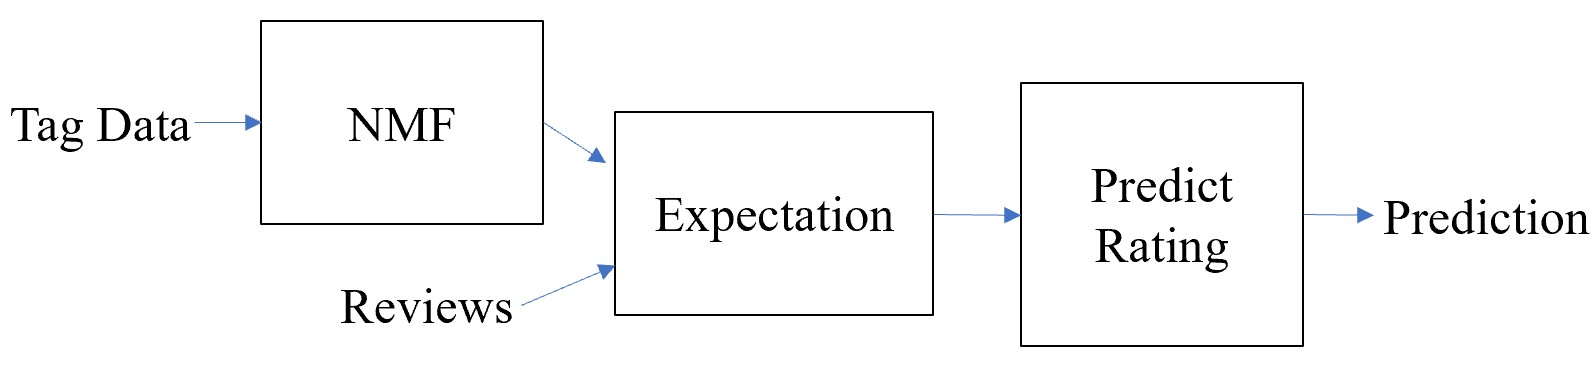
\includegraphics[scale=0.5]{blockdiagram.jpeg}
   \caption{Block diagram of proposed system.}
\end{figure}


The overall architecture for our system is shown in Figure 1.


\section{RESULTS}

\section{CONCLUSION}



\begin{thebibliography}{99}
   \bibitem{c1} test


\end{thebibliography}




\end{document}
